\chapter{Top 5 Takeaways from \emph{The Social Network}}

This lecture unfolds as a countdown, but it is not merely a list. It begins with scale---Mark Zuckerberg as a billionaire at the age of twenty-three---and then asks what sort of entrepreneurial structure could lead to such an outcome. From there the speaker guides us through five connected lessons: persistence after a failed first product, execution beyond ideation, disappointment as redirection, the social cost of scale, and the legal fragility of ownership. The mathematics is necessarily light, because the lecture itself is light on formalism, but a little notation helps us state the institutional logic more clearly.

\section{Opening Frame: An Extreme Outcome and a Program of Lessons}

The lecture begins with a numerical anchor. Zuckerberg is presented not simply as successful, but as successful on an extreme scale and at an unusually early age. The purpose of the number is not to start a valuation exercise. It is to establish that the story is worth studying.

\begin{equation}
a_{\text{Zuckerberg}} = 23
\end{equation}

From that opening fact the speaker turns immediately to method: we are going to extract five takeaways from \emph{The Social Network}. That ordering matters. We do not begin with a doctrine of entrepreneurship and then search for examples. We begin with a concrete case, then let the case unfold into a sequence of lessons.

\section{At Number One: Persistence After the Wrong First Product}

\paragraph{Anecdote.}
The first takeaway does not start with Facebook in its mature form. It starts with FaceMash, which the lecturer presents as Mark Zuckerberg's first idea in college: a service for judging and comparing classmates' attractiveness. The important point is not whether the idea was clever. The point is that it was a failure in business and institutional terms. It led to trouble with Harvard and to academic probation.

\paragraph{Claim.}
From there the lecturer draws a correction to the usual entrepreneurial myth. The first idea is often not the best idea. A false start does not disqualify the founder, and a bad product does not prevent a later, better product from emerging.

\paragraph{Mechanism.}
The lecture then pivots from FaceMash to Facebook. What survives the failure is not the first product itself, but the entrepreneurial motion. The founder keeps moving, and the work is redirected toward something that scales much further.

Once Facebook enters the story, the lecture broadens. We are no longer speaking about the mere existence of a product. We are speaking about the burdens that come with growth. Let us collect those burdens into a single object:
\begin{equation}
B
=
\left\{
\text{awareness},
\text{ user growth},
\text{ investor funding},
\text{ hiring},
\text{ workload},
\text{ product refinement}
\right\}.
\end{equation}

This set \(B\) is not a board equation from the lecture; it is a careful reconstruction of the lecturer's list. He names, in sequence, the need to spread awareness, increase the user base, attract investors to support growth, hire employees, and sustain long hours while improving the product.

That is what gives the first takeaway its real content. Persistence is not a heroic mood. It is the ability to keep working while the shape of the obstacle changes. The early obstacle is product failure. The later obstacles are operational: capital, attention, labor, time, and quality. The lecture's first moral, then, is precise: persistence matters because entrepreneurship is prolonged contact with shifting constraints.

\section{At Number Two: Execution Beats Possession of the Idea}

The second takeaway tightens the argument. It is not enough to survive a bad first attempt; one must also understand what separates a mere idea from a realized business.

\paragraph{Anecdote.}
The lecturer uses the Winklevoss twins and ConnectU for this purpose. They too want a social platform. They too are ambitious. But the speaker's emphasis falls on a different variable: they do not possess the skills necessary to make the idea real, and so they try to bring Mark in to execute it.

\begin{definition}
Let \(I\) denote an idea, let \(E\) denote execution capacity---that is, the skill, organization, and team ability required to build---and let \(O\) denote a realized operating outcome.
\end{definition}

The lecturer's point may then be written in compressed form as
\begin{equation}
I \not\longrightarrow O,
\qquad
I + E \longrightarrow O.
\end{equation}

This notation is deliberately sparse, but it captures the lecture's claim. An idea alone does not become a company simply by being good. The idea must be attached to the means of execution.

The lecture then adds an institutional coda. Although the Winklevoss twins do not build the dominant platform, they do receive a settlement:
\begin{equation}
S_{\text{Winklevoss settlement}} = \$65\,\text{million}.
\end{equation}

That number is important, but only as a coda. The lecturer does not use it to reverse the lesson. He does not conclude that ideation outranks execution after all. Rather, he shows that disputes over who first had the idea can continue even when execution has already decided who built the actual business. The moral of the story stays where the lecturer put it: a great idea without the ability to build remains only an idea.

\section{At Number Three: Not Getting What We Want Can Be a Blessing}

The third takeaway is where the lecture briefly risks losing its footing, and precisely there it becomes most interesting.

\paragraph{Anecdote.}
The speaker begins with the film's story that Mark is broken up with, goes home angry, and creates FaceMash. Then he interrupts his own narrative and says that this was actually false: the movie scene should not be treated as literal historical causation.

That interruption matters. It creates a local tension in the lecture and forces the speaker to say what kind of evidence he thinks he is using.

\subsection{Question \& Answer}

\paragraph{Question.}
If the movie's breakup scene is not historically true, why keep it in the lecture?

\paragraph{Answer.}
Because the lecturer is now treating it as a thematic model, not as a verified historical trigger. The literal event may be wrong, but the pattern remains instructive: a blocked desire or disappointed expectation can redirect effort toward something larger. The speaker is careful here. He preserves the scene's usefulness while withdrawing its factual authority.

\paragraph{Mechanism.}
Once that clarification is in place, the lecturer broadens from the film to a general entrepreneurial structure:
\begin{equation}
\text{blocked outcome}
\;\longrightarrow\;
\text{disruption or failure}
\;\longrightarrow\;
\text{new attempt}
\;\longrightarrow\;
\text{larger opportunity}.
\end{equation}

This is not a law of nature and not a guaranteed update rule. It is a concise way of writing what the lecturer means by saying that when one door closes, another one opens. It is a structure of redirection.

To keep the chain visible on the page, it is useful to draw it in a narrow form.

\begin{figure}
\centering
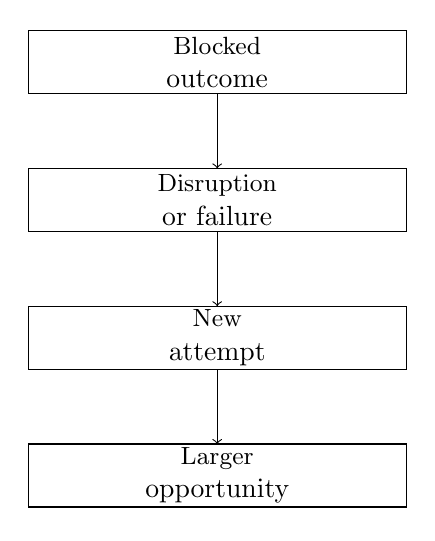
\begin{tikzpicture}[x=1cm,y=1cm]
\draw (-2.4,0.4) rectangle (2.4,-0.4);
\node[align=center] at (0,0) {\small Blocked\\outcome};

\draw (-2.4,-1.35) rectangle (2.4,-2.15);
\node[align=center] at (0,-1.75) {\small Disruption\\or failure};

\draw (-2.4,-3.10) rectangle (2.4,-3.90);
\node[align=center] at (0,-3.50) {\small New\\attempt};

\draw (-2.4,-4.85) rectangle (2.4,-5.65);
\node[align=center] at (0,-5.25) {\small Larger\\opportunity};

\draw[->] (0,-0.4) -- (0,-1.35);
\draw[->] (0,-2.15) -- (0,-3.10);
\draw[->] (0,-3.90) -- (0,-4.85);
\end{tikzpicture}
\end{figure}

The lecturer then adds autobiographical evidence. He says that failed businesses in his own life led to the current opportunity he is working on, namely School of Hard Knocks. That move is structurally important. The lecture does not remain at the level of movie commentary. It uses the film to raise a pattern and then tests that pattern against the speaker's own entrepreneurial life.

\section{At Number Four: Scale Produces Opposition}

The fourth takeaway begins with an intentionally repetitive setup: ``you can't'' several times in succession, and only then the completion of the thought. The completion is that one cannot be ultra successful without creating a few enemies.

That line is easy to trivialize, but we should keep the lecturer's sequence intact. He is not saying merely that successful people are disliked. He is saying that once something grows to large scale, the field around it changes. Visibility rises, rivalry rises, resentment rises, and not all opposition can be negotiated away.

In compact form, the mechanism can be stated as
\begin{equation}
\text{scale}
\;\Longrightarrow\;
\text{visibility}
\;\Longrightarrow\;
\text{opposition}.
\end{equation}

Again, this is a reconstruction, not a quoted formula. But it faithfully captures the lecturer's movement from Zuckerberg's enemies to the general claim that one cannot please everyone.

From there the lecture makes a second turn. The speaker does not answer opposition with a fantasy of universal approval. He answers it by narrowing the field of stability. What matters is the inner circle and self-belief. The entrepreneur's task is not to abolish conflict; it is to continue moving while conflict becomes part of the environment. The lecture even pushes the point one step further: if people are hating on us, that may be evidence that we are no longer invisible.

\section{At Number Five: Shares, Dilution, and the Need to Lawyer Up}

The final takeaway is the most institutional of the five, and it is the one place where a small amount of formal notation genuinely clarifies the lesson.

\paragraph{Anecdote.}
The lecture turns to Eduardo Saverin and says that his shares were diluted because he did not really understand what was happening and signed papers blindly. The lecturer's tone sharpens here. He is no longer speaking mainly about mindset or resilience. He is speaking about ownership, signatures, and the possibility that legal structure can undo what entrepreneurial labor has built.

\begin{definition}
If owner \(i\) holds \(s_i\) shares out of a total of \(S\) shares outstanding, we define the owner's fraction of the company by
\begin{equation}
f_i = \frac{s_i}{S}.
\end{equation}
After a transaction or restructuring, we write the new quantities as
\begin{equation}
f_i' = \frac{s_i'}{S'}.
\end{equation}
\end{definition}

At this point the lecture supports a cautious proposition. We do not know the exact cap-table mechanics from the transcript alone, so we should state only the general ownership logic.

\begin{proposition}
If an owner's own share count stays fixed while the total number of shares rises, then the owner's fraction of the company falls. Equivalently, if
\begin{equation}
s_i' = s_i,
\qquad
S' = S + \Delta S,
\qquad
\Delta S > 0,
\end{equation}
then
\begin{equation}
f_i' = \frac{s_i}{S+\Delta S} < \frac{s_i}{S} = f_i.
\end{equation}
\end{proposition}

\begin{proof}
Starting from the post-transaction fraction,
\[
f_i' = \frac{s_i'}{S'} = \frac{s_i}{S+\Delta S}.
\]
Because \(\Delta S>0\), the denominator \(S+\Delta S\) is larger than \(S\). With the same positive numerator \(s_i\), division by the larger denominator produces the smaller fraction. Hence
\[
\frac{s_i}{S+\Delta S} < \frac{s_i}{S}.
\]
The right-hand side is exactly \(f_i\), so \(f_i' < f_i\).
\end{proof}

This gives us the clean mathematical payload of the lecturer's warning. We are not reconstructing the exact Facebook documents, nor are we claiming a specific historical percentage. We are isolating the mechanism that the lecture wants us to notice: ownership can fall even if one still holds shares, provided the denominator changes against us.

A small worked example makes the mechanism visible:
\begin{align}
s_i &= 30, &
S &= 100, &
f_i &= \frac{30}{100} = 0.30,
\\
s_i' &= 30, &
S' &= 200, &
f_i' &= \frac{30}{200} = 0.15.
\end{align}

The owner still owns something, but not the same fraction. That is the point.

\begin{remark}
The lecture supports the qualitative fact of dilution, not the exact legal route by which it occurred. The numerical example above is therefore illustrative only.
\end{remark}

From this point the lecture turns from algebra back to prudence. The mathematics is the shadow of a practical warning. If we are entering a partnership, signing documents, or doing anything that affects shares and ownership, then friendship and brilliance are not enough. Due diligence becomes part of the entrepreneurial craft.

\begin{itemize}
\item We must understand what is being signed.
\item We must separate friendship from ownership structure.
\item We must treat partnership documents as business instruments, not as tokens of goodwill.
\item We must get legal counsel before signing away rights that affect shares, control, or future upside.
\end{itemize}

This is why the final lesson lands so hard. The earlier takeaways teach us how to keep moving. The last one teaches us how not to lose the thing we have built once paper, capital, and governance enter the picture.

\section{Summary}

The lecture closes by briefly gathering the five takeaways and recommending the film. We may do the same in more deliberate terms.

\begin{enumerate}
\item A failed first product may be a wrong beginning rather than a final verdict.
\item An idea is not a business until execution gives it operative form.
\item A disappointed path may redirect effort toward a larger opportunity.
\item Scale brings opposition, so the entrepreneur cannot rely on universal approval.
\item Ownership is vulnerable to legal structure, and so diligence must accompany ambition.
\end{enumerate}

Taken in order, these are not disconnected slogans. They form a progression. We begin with a false start, we pass to execution, we reinterpret disappointment, we absorb the social cost of scale, and we end by protecting the legal and financial structure of the enterprise itself. That is the lecture's real rhythm, and it is why the countdown works: each lesson answers a different failure mode of entrepreneurship while still pointing toward the same larger question, namely how a venture survives long enough to become durable.